%!TEX root = ../BoYu-Dissertation.tex
\graphicspath{{Figures/}}

\chapter{An Integrated Conceptual Model of Awareness} % (fold)
\label{cha:the_conceptual_framework}
In this chapter, we propose an integrated conceptual model of awareness in large-scale distributed collaborative activities that can satisfy the general requirements identified in Section \ref{sec:discussion}:

\begin{enumerate}
	\item The conceptual model should be able to account for awareness at both the individual and the team levels (\emph{REQ1}).
	\item It should be able to account for how the awareness is distributed across multiple team members, and meanwhile can interact with each other to achieve compatibility (\emph{REQ2}). 
	\item Awareness should be described in reference to activities that the actors are made aware of (\emph{REQ3}).
\end{enumerate}

To satisfy \emph{REQ3}, we build the model of awareness on top of an underlying model of collaborative activities. The activity model plays two important roles to understand the awareness phenomena. First, the three constructs of the activity model, i.e. activity, local scope, and dependency, provide the basis to explain the distributed and dynamic nature of the awareness phenomena (\emph{REQ2}). Second, the activity model is used to understand the development of awareness at both the individual and team levels (\emph{REQ1}). At the individual level, it is used to explain the various cognitive processes that are associated with an individual to achieve and develop individual awareness. At the collaborative level, it accounts for the team processes through which team members interact with each other and mesh their individual awareness together to achieve collaborative awareness. 

In the following of this chapter, we provide the details of our conceptual model in three steps: we first describe the underlying model of collaborative activities in Section \ref{sec:a_model_of_collaborative_activities}; then we use the activity model to characterize the awareness phenomena in large-scale distributed collaborative activities (Section \ref{sec:awareness_requirements}); last we describe the awareness processes through which the collaborative awareness is developed (Section \ref{sec:awareness_processes}).

\section{A model of collaborative activities} % (fold)
\label{sec:a_model_of_collaborative_activities}
Our model of large-scale distributed collaborative activities is built on top of three interrelated constructs (Figure \ref{fig:model_of_collaborative_activity}):

\begin{enumerate}
	\item We appropriate the concept of \emph{activity} from Activity Theory \cite{nardi1996context} to structure the collaborative work.
	\item Due to the distributed nature of collaborative activities, each team member only engages in a subset of actions in the collaborative work, and forms their respective \emph{local scopes of work}.
	\item Actions in different local scopes of work are interdependent due to various types of \emph{dependencies} among them.
\end{enumerate}

\begin{figure}[htbp] %  figure placement: here, top, bottom, or page
   \centering
   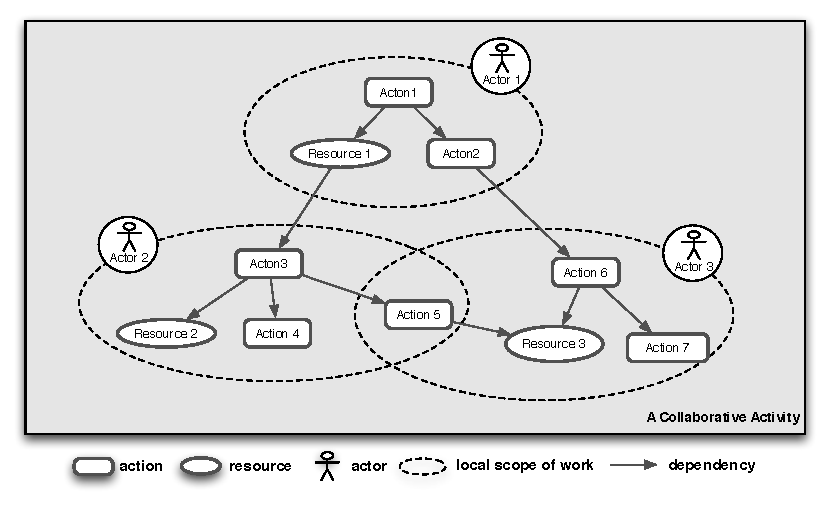
\includegraphics{model_of_collaborative_activity.pdf} 
   \caption{A model of collaborative activities}
   \label{fig:model_of_collaborative_activity}
\end{figure}

In general, a collaborative activity can be defined as a domain model that includes three related sub-models $CoA=\{ER, LS, DEP\}$: the structure of the activity composed of basic entities and their relations $ER$, the set of all actors' local scopes $LS$, and the set of dependencies among activities $DEP$. $ER$ provides the basic vocabulary for defining local scopes $LS$ and dependencies $DEP$. We elaborate on these three components in the rest of this section. 

\subsection{Structure of a collaborative activity} % (fold)
\label{sub:structure_of_a_collaborative_activity}
To model collaborative activities, we subscribe to Activity Theory to conceptualize human activities \cite{nardi1996context}. From this perspective, the structure of a collaborative activity can be defined as several basic entities and relations between them.

\subsubsection{Entities} % (fold)
\label{ssub:entities}
We define three entities that are the basic building blocks in a collaborative activity:
\begin{enumerate}
	\item \textbf{Actions} An action specifies a particular way of doing something. An action can be either basic or complex. A basic action can be directly executed by one or multiple actors. A complex action needs to be decomposed into subsidiary actions. When an action is specified as a sub-component of a higher action, this restricts the higher action to that particular course of doing. An action is assigned to one or more actors who are responsible to perform it. We use $ACT=\{act_1, act_2, ..., act_n\}$ to denote all the actors in a collaborative activity.
   \item \textbf{Actors} are defined as \emph{subjects} intend to and have the capability to perform actions. Actors cast their mental attitudes towards the corresponding action and these internal states are important for the success of an action. $AR=\{ar_1, ar_2, ..., ar_n\}$ is the set of all the actors in a collaborative activity.
   \item \textbf{Resources} are anything that can be used in the performance of an action. One one hand, they can be the \emph{objects} that are manipulated or transformed by the actors while performing actions. On the other hand, they can be the various \emph{tools}, such as instruments, procedures, machines, etc, that are used by the actors to perform their actions. The concepts of object and tool in a collaborative activity are often relative. A tool may be used by an actor in the transformation process of an object, and at the same time the tool itself can be created or transformed by another actor, where it becomes an object of the other actor's action. As a result, we use \emph{resource} as a general term for both \emph{objects} and \emph{tools}. Resources can be can be a material thing (e.g. a vehicle), or intangible (like a rescue plan). $RES=\{res_1, res_2, ..., res_n\}$ denotes the set of resources. 
\end{enumerate}
% subsubsection entities (end)

\subsubsection{Relations} % (fold)
\label{ssub:relations}
The various entities in a collaborative activity are not standalone, rather are connected together to achieve the shared goal of the activity. The relations between these entities can be defined using predicate symbols. For example, predicate symbol $LocatedIn$ can be used to indicate the spatial relation of one entity is inside the second entity. The fact that actor $ar_1$ is in the office $room_3$ can be expressed as $LocatedIn(ar_1, room_3)$. The list of predicate symbols and their meanings are usually domain dependent. However, here we are more interested in defining a subset of relations between these entities that reflect the common characteristics of activity structures, and are used later to define local scopes of work $LS$ and dependencies $DEP$.

\paragraph*{Relations between action and actor} % (fold)
\label{par:relations_between_action_and_actor}
The relations between an action and an actor reflect the levels of participation of the actor in the performance of the action, which can be defined from two aspects: the \emph{intention} of the actor to the action performance, and the \emph{capability} of the actor to perform it. One one hand, the actor participates in an action because of the `motive' or `goal' that arises out of the collaborative activity, and drives the actor to participate in the performance of the action. On the other hand, to what extent the actor can contribute to the action depends on the actor's capability in relation to the action performance. 

We follow the SharedPlans theory \cite{grosz1996collaborative} to define three levels of intentions towards an action that an actor can adopt:

\begin{enumerate}
	\item $Pot.Int$ is used to indicate that an actor would like to adopt an intention that the action is performed, but which has not be committed to yet.
	\item $Int.Th$ represents an actor's intention that the action should be performed.
	\item $Int.To$ is used to express an actor's intention to perform the action.
\end{enumerate}

 The major difference between these three is the level of commitment the actor has on the action. $Pot.Int(ar_1, act_1)$ indicates that actor $ar_1$ is considering adopting the intention that the action $act_1$ should be performed, but has not yet committed to it. $Int.Th(ar_1, act_1)$ indicates that $ar_1$ has intended that $act_1$ should be successfully performed. In this case, $ar_1$ may help other actors to get it done, or avoid resource conflicts, but does not directly perform $act_1$. In the case of $Int.To(ar_1, act_1)$, $ar_1$ has full commitment to perform $act_1$, i.e. $ar_1$ directly participates in the performance of $act_1$.

The \emph{capability} of an actor to perform an action can also be defined at three different levels:

\begin{enumerate}
	\item $Knows$ is used to indicate that the actor has the knowledge about how to perform the action, i.e. the actor knows how to decompose the action into subsidiary actions or basic operations.
	\item $Able$ indicates that the actor has the ability (e.g. expertise, skills) to perform the action.
	\item $Workable$ indicates that the actor can actually perform the action as all the pre-conditions have been satisfied, such as the availability of required resources.
\end{enumerate}

These three relations describe different levels of capability of an actor on an action. $Knows(ar_1, act_1)$ merely says that $ar_1$ knows how to perform $act_1$, but may not be able to perform it. For example, a blind man may know how to drive a car, but is unable to drive it. $Able(ar_1, act_1)$ indicates that $ar_1$ has the ability to perform $act_1$, but it does not necessarily mean the actor can actually perform it. A man who is able to drive the car does not have the key, and hence he cannot actually drive it. $Workable(ar_1, act_1)$ defines the highest level of capability, as $ar_1$ can meet all the constraints and actually perform $act_1$.
% paragraph relations_between_action_and_actor (end)

\paragraph*{Relations between actions} % (fold)
\label{par:relations_between_actions}
An important characteristic of actions is that they can be either \emph{basic} or \emph{complex}. A \emph{basic} action can be directly executed. A \emph{complex} action, however, has to be decomposed into subsidiary actions. The relations between an action and its subsidiary actions can be represented by the predicate $Sub.Act$. $Sub.Act(act_1, act_2)$ indicates that $act_1$ is a subsidiary action of performing $act_2$ within the current plan. $Sub.Act$ only indicates the relation between these two actions under the context of current plan. If the plan is changed, the relationship may no longer hold.

Besides the \emph{decomposition} relation, the actions can also be related by the \emph{precedence} relation. $Precedes$ defines the temporal order of performing two actions, i.e. $Precedes(act_1, act_2)$ indicates that $act_1$ must be performed before $act_2$. 
% paragraph relations_between_actions (end)

\paragraph*{Relations between action and resource} % (fold)
\label{par:relations_between_action_and_resource}
The relations between an action and a resource can be identified depending on the role of the resource in the action performance. One one hand, the resource can be a \emph{tool} that is used in the performance of an action. On the other hand, the resource can be the \emph{object} that is manipulated or transformed during the action performance. We use two predicates, $Consumes$ and $Produces$ to define the relations between an action and a resource. $Consumes(act_1, res_1)$ refers to the situation that the performance of action $act_1$ requires the use of resource $res_1$  (as a \emph{tool}). $Produces(act_1, res_1)$ indicates that the performance of $act_1$ will manipulate the resource $res_1$, or make the resource ready for other actions (as an \emph{object}).
% paragraph relations_between_action_and_resource (end)
% subsubsection relations (end)
% subsection structure_of_a_collaborative_activity (end)

\subsection{Local scope of work} % (fold)
\label{sub:local_scope_of_work}
Within a large-scale collaborative environment, a good number of actions can be identified. However, Each actor usually only engages in a small set of them. In fact, one of the fundamental goals for collaboration is to divide the labor so that a complex problem can be decoupled into a set of smaller ones that are much easier to manage and tackle by individuals \cite{schmidt1992taking}. One result of the division of labor is that the collaborative work of is distributed in the sense that each actor only needs to work on a small set of actions that are suitable for their roles, skills, and experience. To characterize the distributed nature of collaborative activities, we define the \textbf{local scope of work} for each actor as the set of actions that the actor participates in.

Because the participation of an actor in an action can be defined using the \emph{intention} and \emph{capability} relations (Section \ref{ssub:relations}), the local scope of work for an actor can be identified as follow. 

\begin{enumerate}
	\item The \emph{intention} relations are used to define the set of actions that an actor has intention towards their performance. This set of actions form the sub-space of the collaborative activity that the actor is willing to work on, we call it \emph{local scope of intention}. Formally, the \emph{local scope of intention} for an actor $LSI(ar)$ is defined as a set of tuples, and each tuple includes three elements: the actor, the action, and the intention relation between them:
		\begin{align*} 
			LSI(ar) = \{<ar, act, rel(ar, act)>\}
		\end{align*}
		where $act\in ACT$ and $rel\in \{Pos.Int, Int.Th, Int.To, Perform\}$.
	\item The \emph{capability} relations define the set of actions that the actor have certain level of capability to work on. This set of actions form the sub-space of the collaborative activity that the actor can work on, we call it \emph{local scope of capability}. The \emph{local scope of capability} for an actor $LSC(ar)$ is defined as:
		\begin{align*} 
			LSC(ar) = \{<ar, act, rel(ar, act)>\}
		\end{align*}
		where $act\in ACT$ and $rel\in \{Knows, Able, Workable\}$.
\end{enumerate}

The whole \emph{local scope of work} for an actor is then defined as the union of these two sub-spaces defined by the \emph{intention} and \emph{capability} relations (Figure \ref{fig:local_scope}):
\begin{align*} 
	LS(ar) = LSI(ar) \cup LSC(ar)
\end{align*}

\begin{figure}[htbp] %  figure placement: here, top, bottom, or page
   \centering
   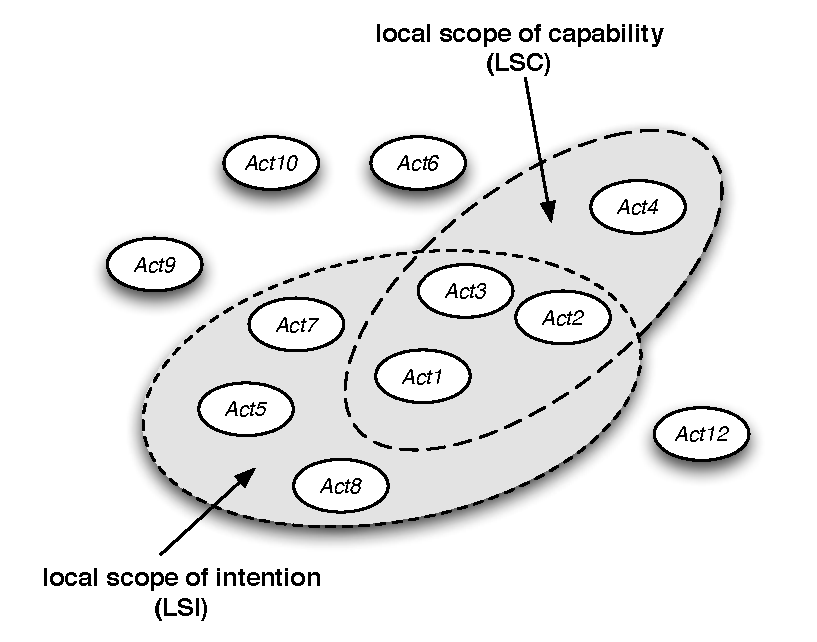
\includegraphics[width=3.5in]{local_scope.pdf} 
   \caption{Local scope of work}
   \label{fig:local_scope}
\end{figure}

The actions within an actor's $LS$ can have different implications on the actor. The actions within the intersect of these two sub-spaces (e.g. $Act1,Act2,Act3$ in Figure \ref{fig:local_scope}) are these that the actor actively participates in because the actor both has certain level of intention and capability towards their performance. The actions within $LSI$, but outside $LSC$ (e.g. $Act5,Act7,Act8$) are these that the actor may need help from other actors as the actor intends that they should be performed, but does not have the necessary capability to do it. The actions outside $LSI$, but inside $LSC$ (e.g. $Act4$) are where the actor can offer help to other actors, even though the action is not initially intended by the actor.

An important property of the \emph{local scope of work} is that local scopes of different actors can overlap with each other. It is common that one action falls into local scopes of multiple actors, even though it may have different implications on these actors. Multiple actors may intend to perform the same action together as a subgroup. The action that is initially intended by one actor may actually be performed by another actor. The different actors may contribute to the same action differently, as one actor contributes the knowledge about how to decompose it in to sub-actions, and the other actor then performs these sub-actions. In all these situations, there are some actions reside in multiple actors' local scopes of work. Actually, these shared actions across overlapping local scopes of work play an important role in understanding the compatibility of awareness that we will discuss in next section.
% subsection local_scope_of_work (end)

\subsection{Dependency} % (fold)
\label{sub:dependency}
Although actions are largely distributed and belong to local scopes of different actors, they cannot be performed without interacting with each other. The \emph{dependencies} between actions represent the knowledge about why and how the actions depend on each other towards the accomplishment of the overall collaborative activity. While local scopes of work divide the actions in a collaborative activity into multiple parts so that each actor can only work on a small portion of it, dependencies show how distinct actions in different local scopes can still be related to each other.

In general, a dependency is defined as a meta-predicate ($DEP$) on two actions ($act_1$, $act_2$) and a proposition $p$, where the performance of $act_1$ depends on the performance of $act_2$ because of some proposition $p$, and is denoted by $DEP(act_1, act_2, p)$. We follow the terms used in \cite{yu1993actor} to call the depending entity $act_1$ the \emph{depender}, and the entity that is depended upon $act_2$ the \emph{dependee}, and the proposition representing the dependency relation \emph{dependum}.

Based on the various types of relations between actions and resources, we can model three types of dependencies that have been recognized in the literature: temporal dependencies, resource dependencies, and goal dependencies.

\paragraph*{Temporal dependencies} % (fold)
\label{par:temporal_dependencies}
Different actions in a collaborative activity might be interdependent due to the constraint of ordering them in a certain order \cite{sikora1998a}. The predicate $Precedes$ can be used to define the temporal dependency between actions, i.e. the performance of $act_2$ as \emph{depender} depends on the performance of $act_1$ as \emph{dependee}, because $act_1$ is a pre-requisite action that must have been completed at the time when $a_2$ is performed. $Precedes(act_1, act_2)$ is the \emph{dependum} in this case.
\begin{align*} 
	 DEP(act_2, act_1, Precede(act_1, act_2))
\end{align*}
% paragraph temporal_dependencies (end)

\paragraph*{Resource dependencies} % (fold)
\label{par:resource_dependencies}
Resource related dependencies can be analyzed in terms of common resources that are involved in multiple actions. Different patterns of use of the common resources by the actions will result in different kinds of resource dependencies. Malone et al. \cite{malone1994interdisciplinary} classify three types of resource dependencies as shown in Figure \ref{fig:resource_deps}, which can be defined using the predicates $Consumes$ and $Produces$:

\begin{figure}[htbp] %  figure placement: here, top, bottom, or page
   \centering
   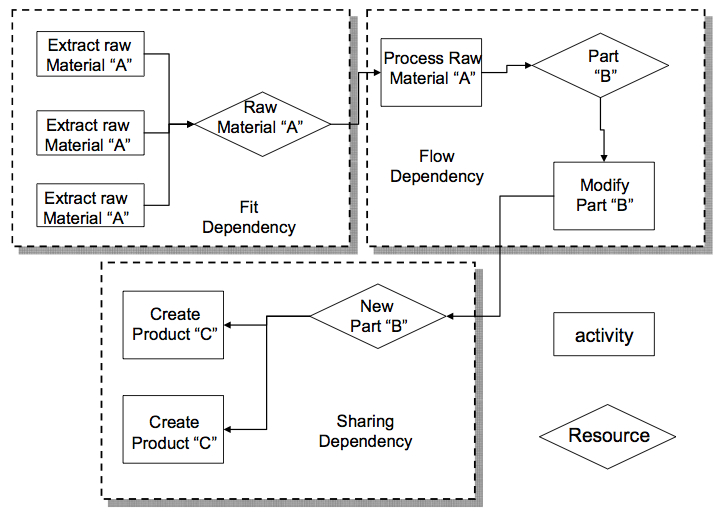
\includegraphics[width=4.5in]{resource_deps.jpg} 
   \caption{Types of resource dependencies \cite{malone1994interdisciplinary}}
   \label{fig:resource_deps}
\end{figure}

\begin{enumerate}
	\item A \emph{fit dependency} occurs when two actions ($act_1$, $act_2$) collectively produce the same resource ($res_1$). In this case, the two actions  are mutually dependent on each other, i.e. both can be \emph{depender} and \emph{dependee} at the same time. The \emph{dependum} is the combination of two predicates: $Produces(act_1, res_1)$ and $Produces(act_2, res_1)$.
		\begin{align*} 
			 DEP(act_1, act_2, Produces(act_1, res_1) \land Produces(act_2, res_1))\\
			 DEP(act_2, act_1, Produces(act_1, res_1) \land Produces(act_2, res_1))
		\end{align*}
	\item A \emph{flow dependency} arises whenever one action $act_1$ produces a resource $res_1$ that is used by another action $act_2$, i.e. the performance of the action $act_2$ as \emph{depender} depends on the performance of the action $act_1$ as \emph{dependee}, because of the two predicates: $Produces(act_1, res_1)$ and $Consumes(act_2, res_1)$.
		\begin{align*} 
			 DEP(act_2, act_1, Produces(act_1, res_1) \land Consumes(act_2, res_1))
		\end{align*}
	\item A \emph{sharing dependency} arises whenever two actions use the same resource. Similar to a fit dependency, the two actions are mutually dependent on each other, because of the two predicates: $Consumes(act_1, res_1)$ and $Consumes(act_2, res_1)$.
	\begin{align*} 
		 DEP(act_1, act_2, Consumes(act_1, res_1) \land Consumes(act_2, res_1))\\
		 DEP(act_2, act_1, Consumes(act_1, res_1) \land Consumes(act_2, res_1))
	\end{align*}
\end{enumerate}
% paragraph resource_dependencies (end)

\paragraph*{Goal dependencies} % (fold)
\label{par:goal_dependencies}
A goal dependency reflects the fact that one action depends on the other action to bring about a certain state in the world. Goal dependency is usually characterized by the decomposition relation between two actions, i.e. action $A$ depends on the other action $B$ because $B$ is a means to achieve a subsidiary goal that must be satisfied in order to perform $A$.

The predicate $Sub.Act$ can be used to define the goal decomposition dependency between two actions. It indicates that action $act_2$ depends on action $act_1$ because $act_1$ is a subsidiary action that must have been completed to achieve $act_2$ in current collaborative activity, i.e. $Sub.Act(act_1, act_2)$
\begin{align*} 
	 DEP(act_2, act_1, Sub.Act(act_1, act_2))
\end{align*}
% paragraph goal_dependencies (end)
% subsection dependency (end)

\subsection{Development of a collaborative activity} % (fold)
\label{sub:development_of_a_collaborative_activity}
As argued in Activity Theory \cite{nardi1996context}, the collaborative activities are not static or rigid, but rather they and their elements are under continuous change and development. This becomes even more significant in large-scale distributed collaborative activities where the actors work in dynamic settings that entail frequent changes in the environment. As argued by Carroll et al. \cite{carroll2006a}, in these open-ended collaborative activities, the `normal' plans of shared activities cannot be precisely specified in advance, and actions and roles cannot be rigidly a priori. As a result, the model of collaborative activities should incorporates several important developmental trajectories:

\begin{enumerate}
 	\item Goal elaboration \cite{Grosz2006}. The development of a collaborative activity usually involves the top-down goal decomposition in which the shared activity is elaborated into multiple actions to complete it. 
 	\item Opportunistic plan revisions \cite{suchman1987plans}. Even after the plan of the shared activity has been identified, some part of the plan may have to be revisited and revised because of the changes in the environment.
 	\item Role transfer \cite{Turoff2004}. In some dynamic situations, it is impossible to predict who will undertake what specific role. Actor may have to perform actions that are outside their initial responsibilities.
 \end{enumerate} 

Because of these developmental trajectories that may occur in a collaborative activity, all the constructs in our model of the collaborative activity can be under continuous change. 
\begin{enumerate}
	\item First, the basic entities and rations in the collaborative activity may be changed. New actions or resources may be added to the model as the plan is developed or revised. The relations between actions and resources may be changed because the same resource is assigned to different actions at different stages of the collaboration.
	\item Second, the local scopes of work are also dynamic.  The local scope of an actor may be expanded as the actor elaborates on the plan of an action, or it can include different sets of actions as the role of the actor is transferred.
	\item Last, the patterns of dependencies among actions are also quite volatile. While two actions may stay the same during the development, new dependency relation may be cast on them because of the possibility of re-planning.
\end{enumerate}
% subsection development_of_a_collaborative_activity (end)
% section a_model_of_collaborative_activities (end)

\section{Characteristics of awareness} % (fold)
\label{sec:awareness_requirements}
The purpose of modeling collaborative activities in previous section is to structure the awareness phenomena on top of it, based on the assumption that any need for the actors to acquire and maintain awareness in a collaborative activity arises out of their need to perform actions \cite{schmidt2002a}. That is to say, what actors are supposedly aware of depends on how they are acting in the collaborative activity. The alignment of awareness phenomena and the underlying activity model allows us to identify three important characteristics of awareness in large-scale distributed collaboration.

\subsection{Partiality of individual awareness} % (fold)
\label{sub:partiality_of_awareness}
The first characteristic of awareness is based on the concept of local scope of work. The idea is that, since each actor only engages in a small set of actions in a large-scale collaborative environment, the actor does not need to fully understand every detail of the whole situation. Instead, the information that an actor should be aware of is only partial, depending on whether it is related to the actions within the actor's local scope of work. An actor would be aware of the information that ascertains or changes the state, progress, direction of one's own work; of the occurrences that makes one's own work more urgent or less; of things that necessitate changes to the intended course of actions to mesh with the unfolding work of others, etc \cite{schmidt2002a}. All of these awareness requirements are motivated and constrained by the actor's local scope of work.

Figure \ref{fig:partiality_of_awareness} illustrates the idea of partiality of individual awareness in a collaborative activity, where each actor only needs to take heed of a partial set of awareness elements that arise out of the actor's corresponding local scope of work. Even though one action can belong to multiple actors' local scopes, the actors may be interested in different aspects of the same action and hence each actor's individual awareness is unique and used for their own work.

\begin{figure}[htbp] %  figure placement: here, top, bottom, or page
   \centering
   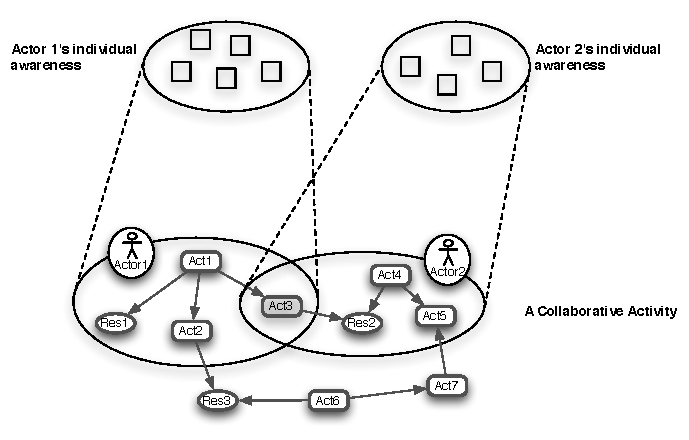
\includegraphics{partiality_of_awareness.pdf} 
   \caption{Partiality of individual awareness}
   \label{fig:partiality_of_awareness}
\end{figure}

The partiality of individual awareness is related to existing theories about local reasoning \cite{Benerecetti2000,ghidini2001local}, which argue that a human actor's reasoning is often based on `local' facts that form the individual's cognitive context \cite{Benerecetti2000}. Such a context is local because it usually only includes information that is potentially relevant to the individual's tasks at hand. Hence, a significant advantage of partitioning the awareness space based on the local scopes of work is that it makes each actor's reasoning more efficient by reducing the number of potential knowledge elements that need to be taken into account \cite{ghidini2001local}.  
% subsection partiality_of_awareness (end)

\subsection{Compatibility of awareness} % (fold)
\label{sub:compatibility_of_awareness}
However, because of the relations among different actors' local scopes of work, the awareness phenomena in large-scale distributed collaboration is not simply equivalent to the partition of the collaborative awareness space into separate individual awareness spaces. Rather, the actors' individual awareness needs to be coordinated so as to achieve the \emph{compatibility} that is collectively needed for the overall team to perform the collaborative task successfully. The requirement for compatible awareness among multiple actors can be accounted for by two typical patterns in the activity model: the overlaps between local scopes of work, and the dependencies across local scopes (Figure \ref{fig:compatibility_of_awareness}).

\begin{figure}[htbp] %  figure placement: here, top, bottom, or page
   \centering
   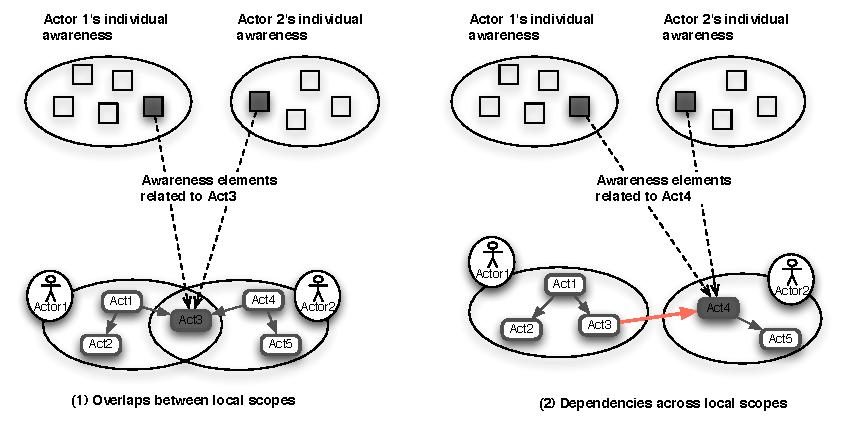
\includegraphics{compatibility_of_awareness.pdf} 
   \caption{Compatibility of awareness}
   \label{fig:compatibility_of_awareness}
\end{figure}

\paragraph*{Overlaps between local scopes} % (fold)
\label{par:overlaps_between_local_scopes}
Although the actions in different actors' local scopes of work can be quite different, it is quite common that some actions sit in between local scopes of different actors as boundary objects. Multiple actors may work as a subgroup to perform the same action together, or an actor delegates an intended action to another actor who has the capability to perform it. These boundary objects pose the need for the actors to achieve compatibility. The actors working on the same action need to share their individual interpretations of the action with each other to make sure they are on the same page. The actor who is performing the delegated action needs to update the status to the actor who adopts the initial intention so that he/she knows what to expect. 
% paragraph overlaps_between_local_scopes (end)

\paragraph*{Dependencies across local scopes} % (fold)
 \label{par:dependencies_across_local_scopes}
 The second driving force to achieve compatible awareness comes from dependencies that can connect actions from two disjoint local scopes of work. For example, in Figure \ref{fig:compatibility_of_awareness}(b), because the action $Act3$ of $Actor1$ depends on $Actor2$'s action $Act4$, $Actor1$ will also be interested in knowing the information related to $Act4$, such as the fact that $Act4$ has been successfully completed or it encounters problems. In such case, even though $Act4$ is outside $Actor1$'s local scope, $Actor1$ still wants to be aware of aspects of $Act4$ that are likely to impact his/her own action $Act3$ due to the dependency relation between these two actions.
 % paragraph dependencies_across_local_scopes (end) 

The compatibility of awareness between actors is achieved by awareness \emph{transactions} \cite{Salmon2010}. An awareness transaction represents an exchange of individual awareness between two actors. One actor receives information and interprets it. If the result of the interpretation is related to the shared action with the other actor, or it is a dependee of the other actor's action, it is passed to the other actor. In this way, the compatibility between the two actors is achieved. In next section, we will provide more detail about how awareness transactions can be achieved through team processes. 
% subsection compatibility_of_awareness (end)

\subsection{Dynamics of awareness} % (fold)
\label{sub:dynamics_of_awareness}
As we pointed out in Section \ref{sub:development_of_a_collaborative_activity}, the elements and relations, local scopes of work, and dependencies are all under continuous change and development in large-scale distributed collaborative activities. As a result, we can postulate that an actor's awareness requirement, i.e. the information an actor need to be aware of, also entails frequent changes. The awareness elements that were relevant to the actor may later become irrelevant, as they are related to the action that is no longer part of the actor's local scope of work. New awareness elements may have to be added to the actor's awareness requirement as the local scope expands or new dependency is activated. Figure \ref{fig:dynamics_of_awareness} shows an example of the dynamic of awareness as an actor's local scope of work is changed due to plan development.

\begin{figure}[htbp] %  figure placement: here, top, bottom, or page
   \centering
   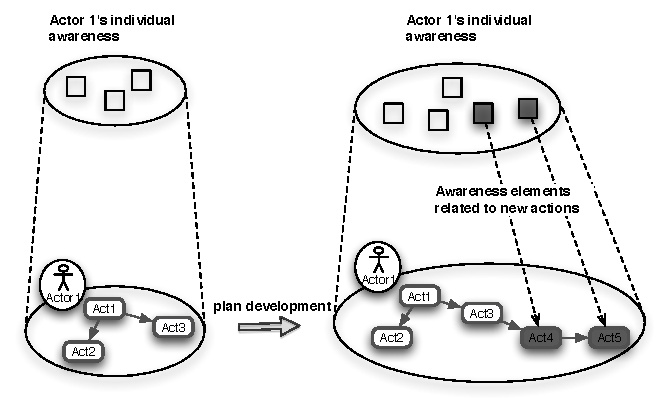
\includegraphics{dynamics_of_awareness.pdf} 
   \caption{Dynamics of awareness}
   \label{fig:dynamics_of_awareness}
\end{figure}

The dynamics of awareness is coupled with the development of the collaborative activity. As we will show in next section, the collaborative awareness and activity are mutually developed through a set of individual and team processes. The actors' awareness requirements are changed as the collaborative activity is developed. Guided by the new awareness requirements, the actors process new awareness information and adjust their behaviors that lead to further development of the collaborative activity. This is very similar to Niesser's perceptual cycle model \cite{neisser1976cognition}, but applies to the collaborative environments.
% subsection dynamics_of_awareness (end)
% section awareness_requirements (end)

\section{Awareness processes} % (fold)
\label{sec:awareness_processes}
Because of the partiality and compatibility of awareness in large-scale distributed collaboration, we believe that awareness is developed at both the individual and team levels. At the individual level, each actor develops his/her own partial awareness through a set of cognitive processes. At the team level, the actors engage in team processes to perform transactions in order to achieve compatible awareness. 

\subsection{Development of individual awareness} % (fold)
\label{sub:development_of_individual_awareness}
At the individual level, each team member develops his/her own awareness in the similar way as described in the Neisser's perceptual cycle model \cite{neisser1976cognition}: the development of awareness starts with the perception of selective elements, which is then interpreted with the help of the actor's existing knowledge. The result of the individual awareness processes then helps the actor to make decisions and perform actions, which generate new awareness elements and trigger another round of awareness processes (Figure \ref{fig:individual_processes}). 

\begin{figure}[htbp] %  figure placement: here, top, bottom, or page
   \centering
   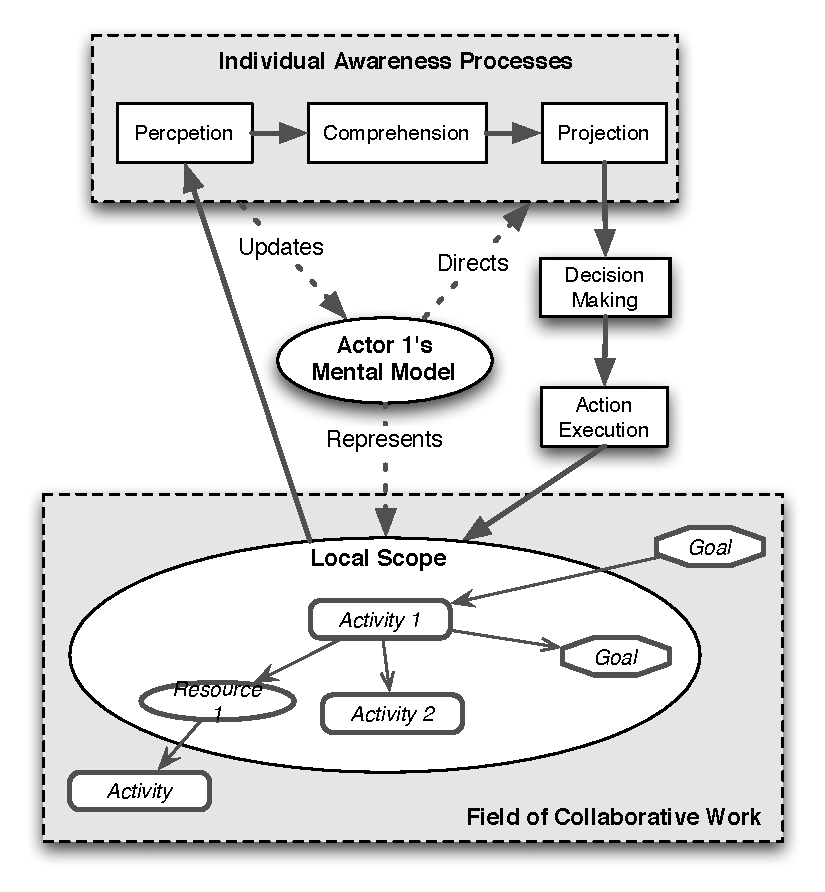
\includegraphics{individual_processes.pdf} 
   \caption{Development of individual awareness}
   \label{fig:individual_processes}
\end{figure}

The major difference in our model from the original perceptual cycle model is that the actor's local scope of work plays important roles in the individual awareness processes:

\begin{enumerate}
	\item \emph{Perception}. An actor must first be able to gather perceptual information in the surrounding situation, and selectively attend to those elements that are most relevant for the task at hand. The perception is constrained by the actor's local scope, i.e. he/she is only interested in awareness information that have explicit or implicit impact on actions in his/her local scope.
   \item \emph{Comprehension}. Comprehension refers to the mental activities where perceived awareness information is processed for the purpose of understanding its meaning in the context of the individual's goals and actions in the local scope, i.e. the actor needs to understand how the perceived information is related to his/her own work.
	\item \emph{Projection}. Projection is the process in which the actor predicts likely future states of the actions in the local scope of work.
\end{enumerate}
% subsection development_of_individual_awareness (end)

\subsection{Development of collaborative awareness} % (fold)
\label{sub:development_of_collaborative_awareness}
The development of awareness at the team level is mediated by the transactions between multiple actors. Transactions allow for the exchange of individual awareness between actors to achieve the compatibility. The development of awareness at the team level usually entails multiple transactions through which actors' individual awareness processes are connected as developmental trajectories.

\subsubsection{Awareness transactions} % (fold)
\label{ssub:awareness_transactions}
An awareness transaction represents an exchange of awareness information between two actors to achieve compatibility. Transactions happen whenever compatibility of individual awareness becomes necessary. If the result of one actor's individual awareness is related to the shared action with the other actor, or is related to the action that the other actor's action depends on, it is exchanged with the other actor through an awareness transaction. We call the first actor the \emph{initiator} of the transaction, and the second actor the \emph{receiver} of the transaction.

Awareness transactions can be achieved by joint effort from both the initiators and receivers through two complementary awareness practices: monitoring and displaying \cite{heath2002a}. One one hand is the initiators display their own actions appropriately visible to other actors, and at the same time the receivers actively monitor the actions of other actors in the collaborative setting. Based on how the effort is divided between initiators and receivers, we can identify three types of awareness transactions.

\paragraph*{Mutual monitoring} % (fold)
\label{par:monitoring}
The first type of awareness transactions refers to the process of actors mutually monitoring the actions of each other in a collaborative environment. The perception of such actions allows the actors to understand how other actors' actions can impact their own actions so as to achieve compatibility. An awareness transaction based on mutual monitoring directly connects two actors' individual awareness processes in the following way (Figure \ref{fig:trans_monitoring}). First, some awareness element in the situation triggers the first actor ($Actor1$)'s individual awareness process, in which $Actor1$ perceives the awareness information, comprehends and projects it. The result of the actor's individual awareness process leads to some action performed by $Actor1$. The performance of the action is then perceived by the other actor ($Actor2$), as $Actor2$ is actively monitoring it. As a result, $Actor2$ starts the individual awareness process to consume the perceived information. In this way, the actors do not need to engage in any explicit team processes, as the transaction is implicitly achieved by the actors' individual perception.

\begin{figure}[htbp] %  figure placement: here, top, bottom, or page
   \centering
   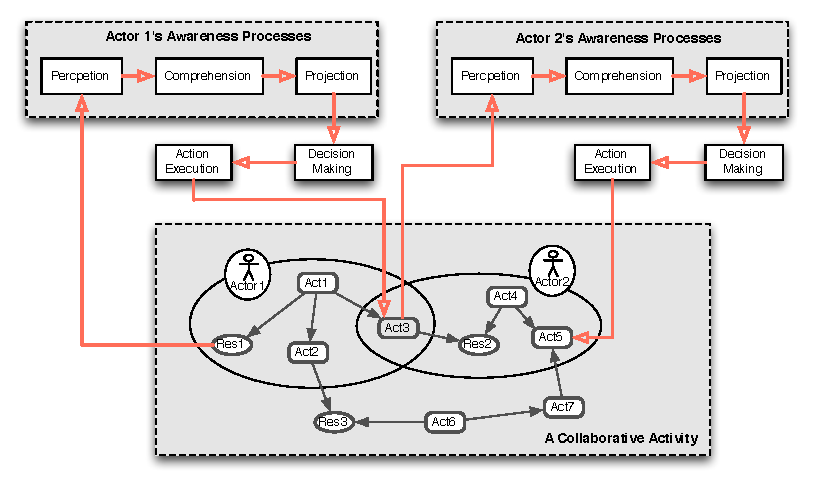
\includegraphics{trans_monitoring.pdf} 
   \caption{Awareness transaction via mutual monitoring}
   \label{fig:trans_monitoring}
\end{figure}

Awareness transactions via mutual monitoring primarily rely on the receivers to perceive the awareness information from the field of collaborative work and assume that the aspects of actors' actions be visible to each other. However, it has two limitations. 
\begin{enumerate}
	\item Without explicit externalization or disclosure, the actors can only monitor external aspects of other actors' actions \cite{Rittenbruch2007}. However, many aspects of human actions are intentional in the sense that the awareness information related to these actions is the state of someone else's mind \cite{carroll2003a}. As a result, the awareness information on these aspects cannot be exchanged merely based on mutual monitoring.
	\item In order to perform the awareness transactions via mutual monitoring, every actor in the collaborative activity needs to spare some attentional resource to each other's actions. When the number of actors and their actions grows significantly, it requires a lot of extra attentions and efforts from the actors.
\end{enumerate}
% paragraph monitoring (end)

\paragraph*{Communication} % (fold)
\label{par:communication}
Alternatively, awareness transactions can be conducted via intentional communications, in which actors explicitly exchange awareness information with their collaborators through direct communications. As shown in Figure \ref{fig:trans_communication}, the first actor ($Actor1$) can explicitly state the result of his/her individual awareness processes, and convey it to the other actor ($Actor2$) who might be interested in knowing it. Upon receiving the communicated information, $Actor2$ starts the individual awareness process to consume it. 

\begin{figure}[htbp] %  figure placement: here, top, bottom, or page
   \centering
   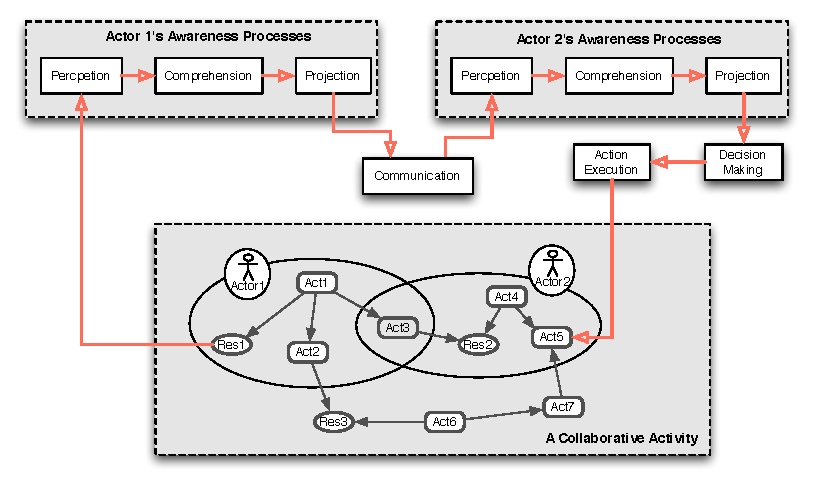
\includegraphics{trans_communication.pdf} 
   \caption{Awareness transaction via communication}
   \label{fig:trans_communication}
\end{figure}

Unlike awareness transactions via mutual monitoring, the transaction cost in the communication process is largely posed on the actor who initiates it. The initiator needs to first create the message that he/she wants to communicate, identifies the collaborators who might be interested in knowing it, and starts the communication. Besides, the communication may be too obtrusive that it causes interruptions on the receivers, as they have to switch their focus from the current line of work in order to consume the information.
% paragraph communication (end)

\paragraph*{Externalization} % (fold)
\label{par:externalization}
Externalization refers to an indirect means to exchanging intentional aspects of awareness among team members. Instead of explicit communication, team members can externalize some intentional aspects of their individual awareness and make them visible to others, so that anyone who is interested in these aspects can perceive them. As shown in Figure \ref{fig:trans_externalization}, $Actor1$ first externalizes the result of his/her individual awareness processes on an action. Instead of communicating it directly to $Actor2$, $Actor1$ attaches it with the action and makes it visible to others. The externalized information is then perceived by $Actor2$, and $Actor2$ starts the individual awareness process to consume the information.

\begin{figure}[htbp] %  figure placement: here, top, bottom, or page
   \centering
   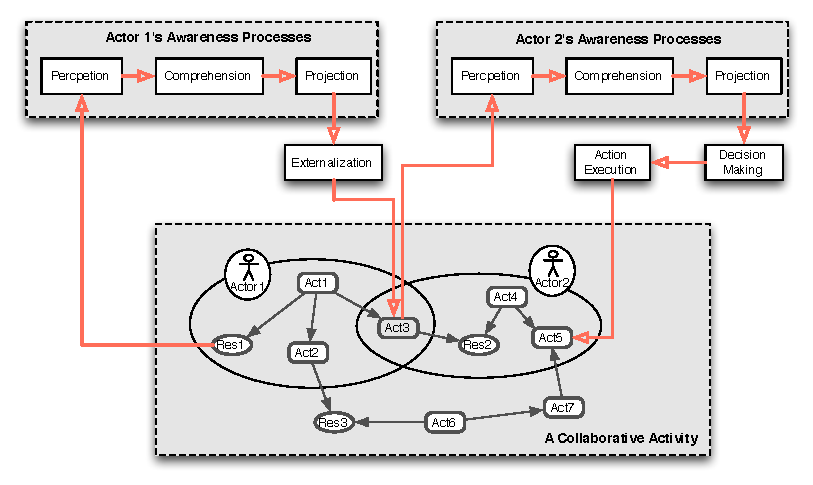
\includegraphics{trans_externalization.pdf} 
   \caption{Awareness transaction via externalization}
   \label{fig:trans_externalization}
\end{figure}

The awareness transactions via externalization balance the efforts between the initiators and the receivers. On one hand, the initiators need to explicitly externalize some intentional aspect of their individual awareness and attach the externalized information with related actions. On the other hand, the actors who are interested in receiving information about these actions need to actively monitor them so that the information can be processed. Comparing with awareness transactions that merely rely on mutual monitoring, the externalization-based awareness transactions can support the exchange of intentional aspects of awareness, such as human actors' intentions to actions, or their interpretations of the situation. Comparing with direct communication, it has a lower level of obtrusiveness as it gives receivers control on when to consume the information.
% paragraph externalization (end)
% subsubsection awareness_transactions (end)

\subsubsection{Developmental trajectories} % (fold)
\label{ssub:developmental_trajectories}
The development of awareness at the team level is seldom achieved by one single awareness transaction, rather most likely to entail a sequence of awareness transactions among multiple actors. In this way, we consider the development of collaborative awareness as developmental trajectories \cite{strauss1993continual} that are triggered by some initial awareness information, and then the awareness knowledge evolves over time, contributed by a series of transactions.

Figure \ref{fig:developmental_trajectory} illustrates the idea of a developmental trajectory including multiple awareness processes. In the beginning, $Actor1$ performs some action $Action1$ in the local scope, which is perceived by $Actor2$, as $Actor2$ is monitoring the status of $Action1$ (a transaction via \emph{mutual monitoring}). Upon receiving the awareness element associated with $Action1$, $Actor2$ develops the individual awareness by interpreting how the awareness element on $Action1$ may impact his/her own work, and leads to some new awareness element that he/she wants to pass to another actor $Actor3$. As a result, $Actor2$ initiates a direct communication with $Actor3$ (a transaction via \emph{communication}), triggering $Actor3$'s individual awareness process to understand the communicated message. The result of $Actor3$'s individual awareness process is externalized as a new awareness element that is attached to a shared action with $Actor4$ (a transaction via \emph{externalization}). As $Actor4$ is monitoring the shared action with $Actor3$, he/she perceives the awareness element passed from $Actor3$, starts the individual awareness process and leads to further changes on his/her action $Action2$.

\begin{figure}[htbp] %  figure placement: here, top, bottom, or page
   \centering
   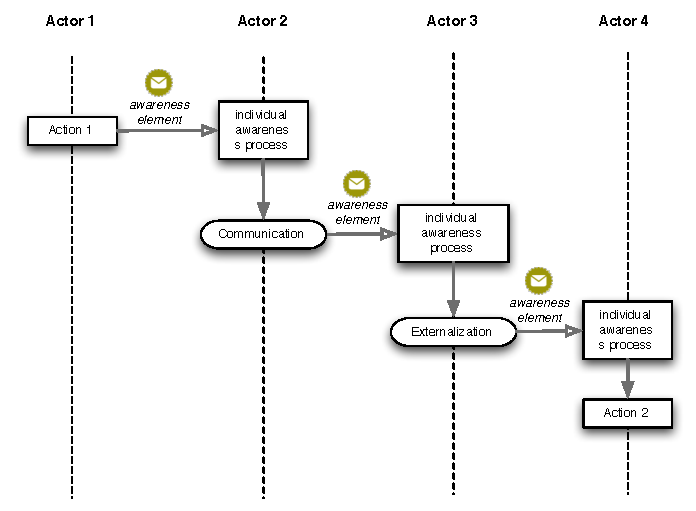
\includegraphics{developmental_trajectory.pdf} 
   \caption{Developmental trajectory of awareness}
   \label{fig:developmental_trajectory}
\end{figure}

Conceptualizing the development of awareness at the team level as developmental trajectories exhibit several important characteristics of the collaborative awareness phenomena:

\begin{enumerate}
	\item The awareness knowledge at the team level is socially constructed through multiple awareness transactions. The awareness element perceived by $Actor3$ is different from the initial information received by $Actor2$, however they are related as the former is built on top of $Actor2$'s interpretation of the latter. In this way, the awareness knowledge is undergoing continuous construction as the initial awareness information is enriched in every awareness transaction.
	\item In one developmental trajectory, different types of awareness transactions can be observed. In the example demonstrated by Figure \ref{fig:developmental_trajectory}, the transaction between $Actor1$ and $Actor2$ is based on mutual monitoring; then $Actor2$ directly communicates the awareness message to $Actor3$; last the transaction from $Actor3$ to $Actor4$ is via externalization. 
	\item The development of awareness is coupled with the development of the collaborative activity. In the example illustrated by Figure \ref{fig:developmental_trajectory}, the whole awareness development is triggered by the performance of some action, i.e. $Action1$. On the other hand, the development of awareness throughout the four actors then leads to $Actor4$ to perform another action, i.e. $Action2$. 
\end{enumerate}
% subsubsection developmental_trajectories (end)
% subsection development_of_collaborative_awareness (end)
% section awareness_processes (end)

\section{Discussion} % (fold)
\label{sec:discussion}
In this chapter, we present our conceptual model of awareness in large-scale distributed collaboration. Our conceptual model is based on the understanding of collaborative activities, from which we identify the major characteristics of the awareness phenomena and elaborate on the awareness processes through which the awareness is developed at both the individual level and the team level.

In Section \ref{sec:understanding_the_awareness_phenomena_in_the_scenario}, we apply the conceptual model in an emergency response scenario to understand the major characteristics and developmental trajectories of the awareness phenomena in large-scale distributed collaborative activities. 

The proposed conceptual framework shows the capabilities to satisfy the three requirements we presented in the beginning of this section.
\begin{enumerate}
	\item First, the conceptual model takes into account the awareness phenomena at both the individual level and team level. Each actor develops their individual awareness through individual cognitive processes and at the same time, the actors engage in team processes to conduct transactions to achieve collaborative awareness.  
	\item Second, the concept of local scope and dependencies allows us to define how the awareness is distributed across multiple actors. The different actors often attend to different sets of actions in their respective local scopes of work (\emph{partiality}). At the same time, the actors' local scopes are often overlapped due to the shared actions, or various dependency relations may occur across multiple local scopes. This drives the occurrence of awareness transactions among multiple actors to achieve \emph{compatibility}.
	\item Last, Our model is built on top of the underlying model of collaborative activities. Our discussion of the major characteristics of awareness phenomena, and the various individual and team processes to develop awareness is centered around the concept of activity, local scopes of work, and dependencies.
\end{enumerate}
% section discussion (end)
% chapter the_conceptual_framework (end)




 

